\documentclass[xcolor=dvipsnames]{beamer}

% Ausgelagerte Praeambel
\mode<presentation> {
   \usetheme{Copenhagen}
   \usecolortheme[named=PineGreen]{structure}
   \setbeamercovered{dynamic}
}

% Sprache und Zeichnsatz
\usepackage[ngerman]{babel} 
\usepackage[latin1]{inputenc}

% font definitions, try \usepackage{ae} instead of the following
% three lines if you don't like this look
\usepackage{mathptmx}
\usepackage[scaled=.90]{helvet}
\usepackage{courier}

% Um Bilder einzufuegen
\usepackage{graphicx} 

\usepackage[T1]{fontenc}

% Titelseiteninformationen
\author[Lukas Ehnle, Jo Klawitter, 
Nikos Moraitakis, Alex Noe, Anas Saber]{Lukas Ehnle, 
Jo Klawitter, Nikos Moraitakis, Alex Noe, Anas Saber}
\institute{KIT, Fakult�t f�r Informatik}
\date{\today} 

 
% This is only inserted into the PDF information catalog. 
\subject{Tutoriumsfolien}
\keywords{PSE10, Research Phase}


% Logo rechts unten einbinden
\pgfdeclareimage[height=0.8cm]{university-logo}{Pictures/KIT-Logo.png}
\logo{\pgfuseimage{university-logo}}


  
% Abschalten der unteren Symbolleiste:
\beamertemplatenavigationsymbolsempty

% If you wish to uncover everything in a step-wise fashion, uncomment
% the following command:
%\beamerdefaultoverlayspecification{<+->}
 


%<[BEGIN]><[BEGIN]><[BEGIN]><[BEGIN]><[BEGIN]><[BEGIN]><[BEGIN]><[BEGIN]>
\begin{document}  %<[BEGIN]><[BEGIN]><[BEGIN]><[BEGIN]><[BEGIN]><[BEGIN]>
%<[BEGIN]><[BEGIN]><[BEGIN]><[BEGIN]><[BEGIN]><[BEGIN]><[BEGIN]><[BEGIN]>

% :-:-:-[ Starteite ]-:-:-:-:-:-:-:-:-:-:-:-:-:-:-:-:-:-:-:-:-:-:-:
\begin{frame}
\begin{center}
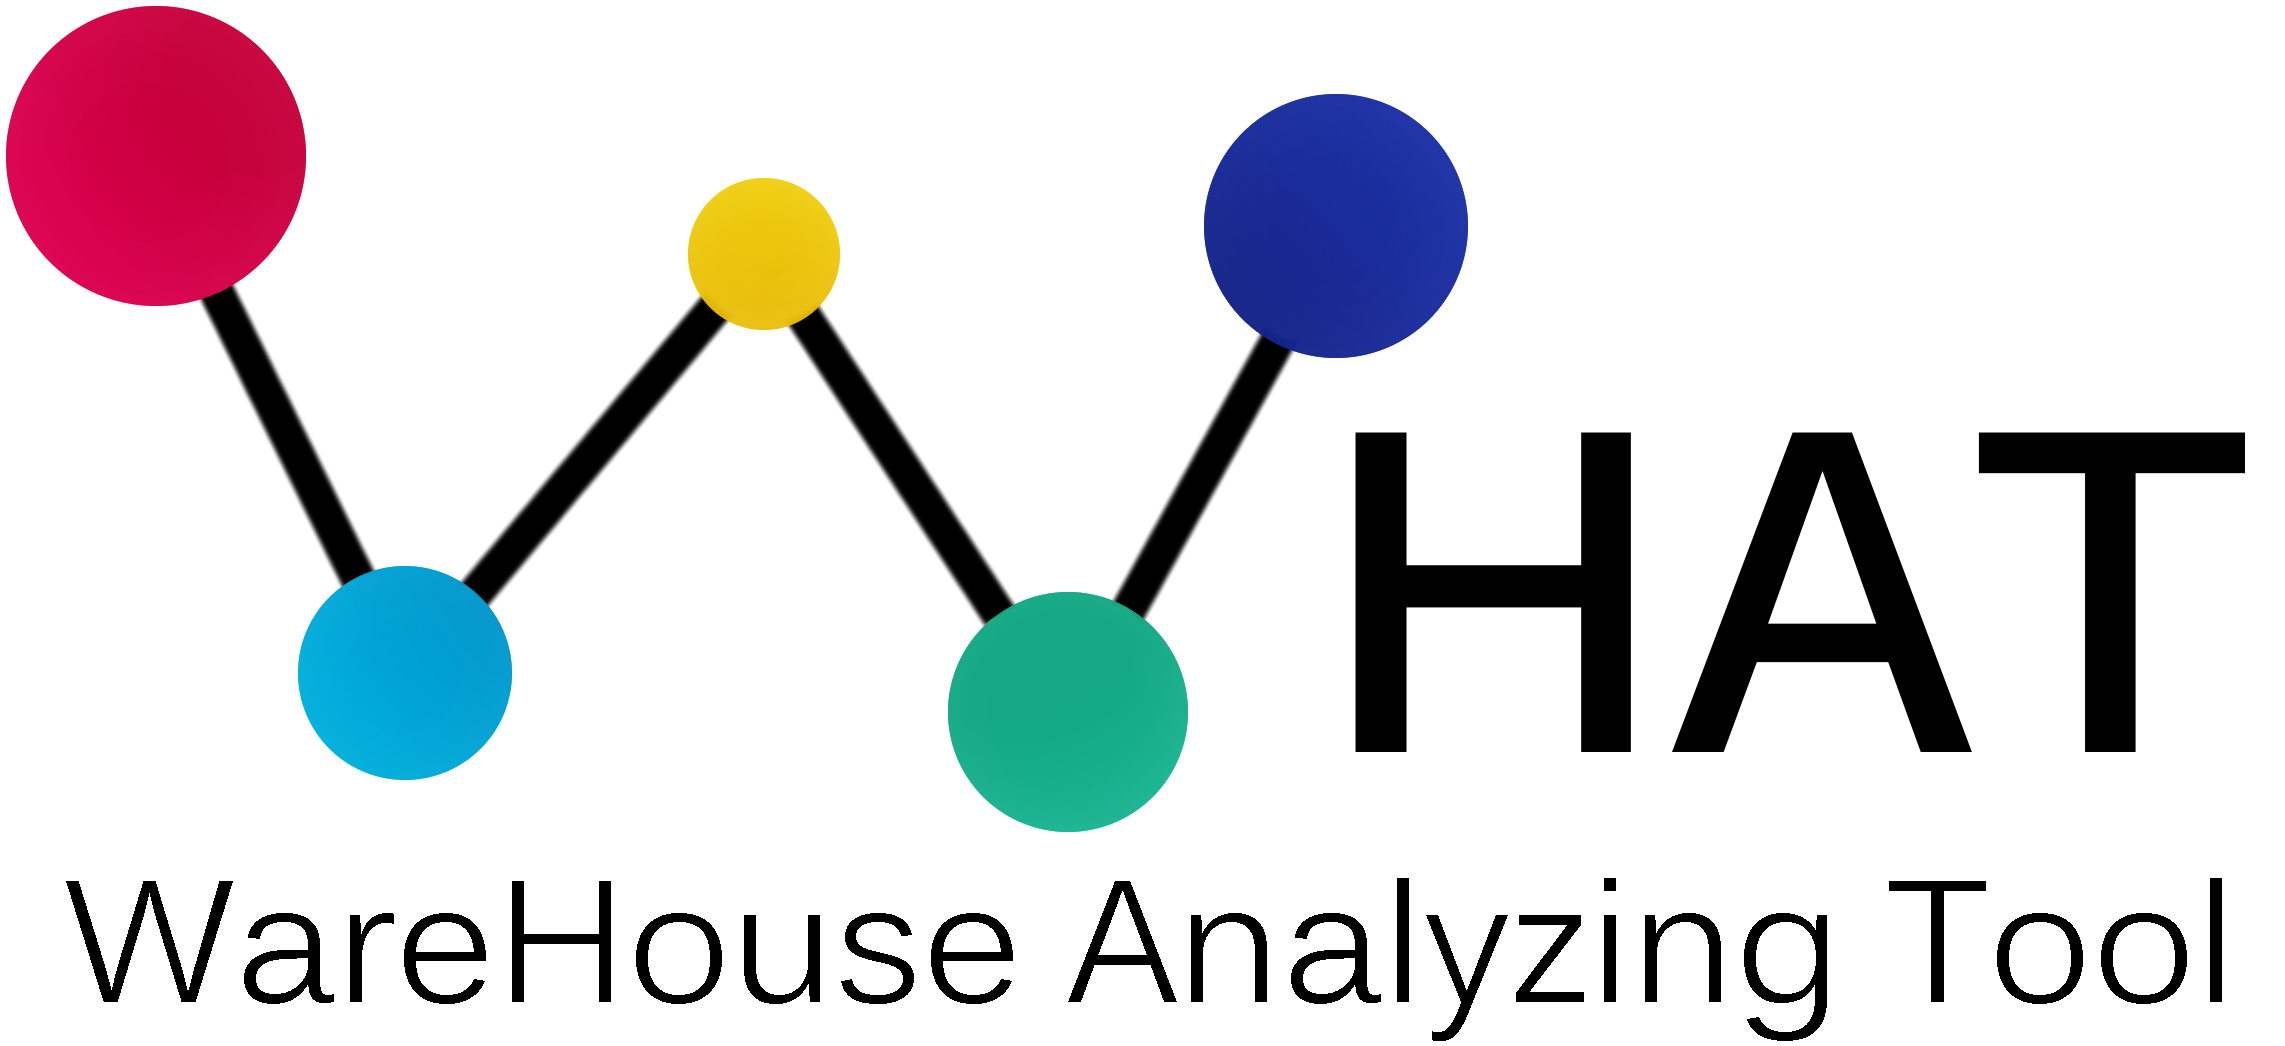
\includegraphics[width =0.7\linewidth]{Pictures/WHAT-Logo2.png}
\end{center}

\end{frame}
% 
% % :-:-:-[ Titelseite ]-:-:-:-:-:-:-:-:-:-:-:-:-:-:-:-:-:-:-:-:-:-:-:
% \begin{frame}
% \titlepage
% \end{frame} 

% % :-:-:-[ Inhaltsverzeichnis ]-:-:-:-:-:-:-:-:-:-:-:-:-:-:-:-:-:-:-:
% \begin{frame}{Content} 
% \tableofcontents%[hideallsubsections]
% \end{frame}


%  - - -[ Folie ]- - - - - - - - - - - - - - - - - - - - - - - - - -
\begin{frame}{task}
\huge{Visualizing and Statistically Analyzing Access Behavior to Scientific Databases}
%\includegraphics[width=1\linewidth]{PicturenameHere.png}

\end{frame}


\begin{frame}{task}
\begin{itemize}
  \item<2-> process data from SkyServer.org server log files
  \item<3-> save data in database
  \item<4-> compute charts
\end{itemize}
\end{frame}

\begin{frame}{csv}
	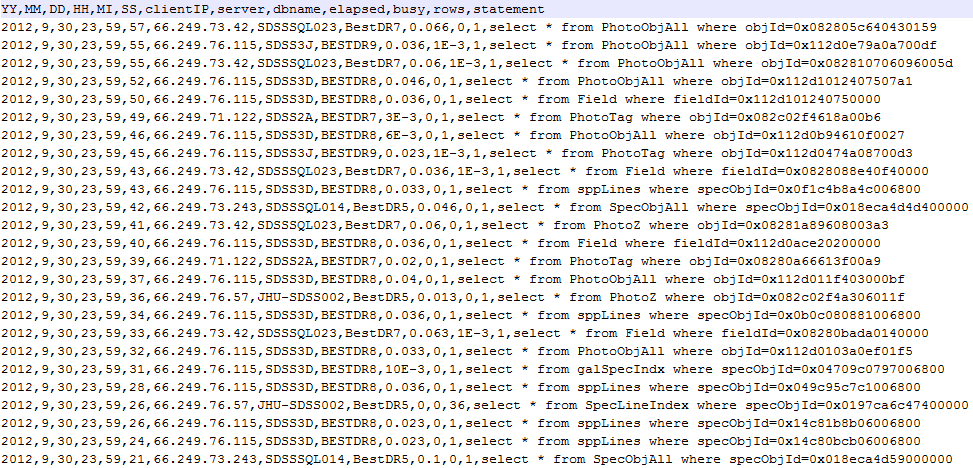
\includegraphics[width=1\linewidth]{Pictures/csv.png}
\end{frame}

\begin{frame}{bubble chart}
	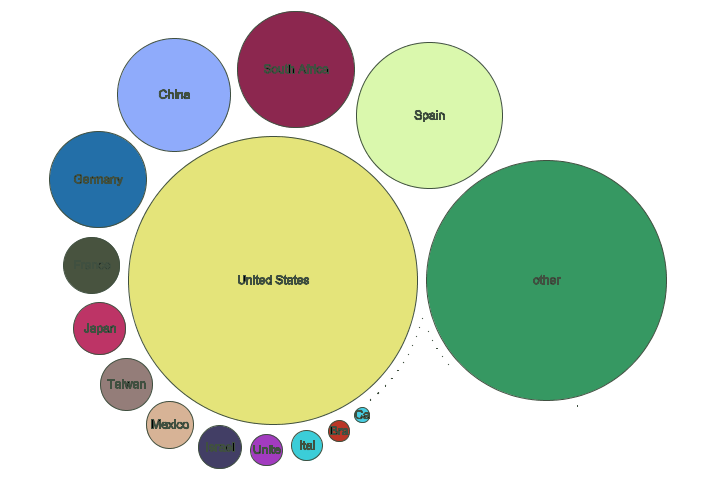
\includegraphics[width=1\linewidth]{Pictures/bubblechart.png}
\end{frame}

\begin{frame}{scatterplot + bubble chart}
	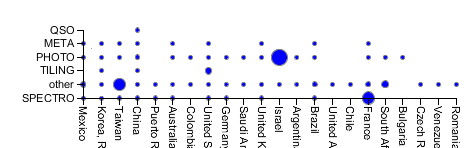
\includegraphics[width=1\linewidth]{Pictures/bubblescatter.png}
\end{frame}

\begin{frame}{purpose}
	Find out:
	\begin{itemize}
		\item<1-> what parts of your servers were accessed,
		\item<2-> when they were accessed,
		\item<3-> and from where in the world
	\end{itemize}
	\uncover<4-> {use e.g. to create a better user expierience}
\end{frame}

\begin{frame}{main functions}
\uncover<1-> WHAT - \textbf{W}are\textbf{H}ouse \textbf{A}nalyzing \textbf{T}ool
	\begin{itemize}
	  \item<2-> process server log files
	  \item<2-> and load data into database
	  \item<3-> choose different chart types
	  \item<4-> compute charts with customizable parameters
	  \item<5-> export charts
	\end{itemize}
\end{frame}

\begin{frame}{}
	\begin{center}
	\huge{project demonstration}
	\end{center}
\end{frame}  

\begin{frame}{client - server model}
	reasoning:
	\begin{itemize}
	  \item<2-> amount of data
	  \item<3-> already present server infrastructure, most likely
	\end{itemize}
\end{frame}

\begin{frame}{client - server model}
	flexibility:
	\begin{itemize}
	  \item<2-> not OS dependant
	  \item<3-> device independant %better term?
	  \item<4-> possibility to provide easy access to others
	\end{itemize}
\end{frame}

\begin{frame}{development goals}
	\begin{itemize}
	  \item<1-> configurable (not only SkyServer)
	  \item<2-> simple user interface
	  \item<3-> extendability
	\end{itemize}
\end{frame}

\begin{frame}{extendability + future development}
	extendability:
	\begin{itemize}
	  \item<2-> more languages
	  \item<3-> extend charts/add new ones
	\end{itemize}
	\uncover<4-> {future development:}
	\begin{itemize}
	  \item<5-> support for olap server
	  \item<6-> more admin functions, e.g. order charts
	  \item<7-> more export formats
	  \item<8-> support for other log file formats
	  \item<9-> support for other data sources
	\end{itemize}
\end{frame}

\begin{frame}{extendability + future development}
	open source: https://github.com/Gruppe14/KIT-PSE
	\newline development documents: https://github.com/Gruppe14/KIT-PSE-Docs
	\newline including this presentation.
	\newline
	\newline JVM version:
	\newline https://www.dropbox.com/sh/c0zm0f0vtli0kxy/l2Ahm8PRB4/KIT-PSE
\end{frame}

\begin{frame}{}
	\begin{center}
	\huge{Questions?}
	\end{center}
\end{frame}  

%  - - -[ Folie ]- - - - - - - - - - - - - - - - - - - - - - - - - -
\begin{frame}{end}

\begin{center}
\huge{Thanks for listening!}
\end{center}


\end{frame}  


%<[END]><[END]><[END]><[END]><[END]><[END]><[END]><[END]><[END]><[END]>
\end{document}       %<[END]><[END]><[END]><[END]><[END]><[END]><[END]>
%<[END]><[END]><[END]><[END]><[END]><[END]><[END]><[END]><[END]><[END]>